\documentclass[12pt]{article}
\input{bayesuvius.sty}
\begin{document}

\begin{figure}[h!]\centering
\begin{minipage}{.4\linewidth}
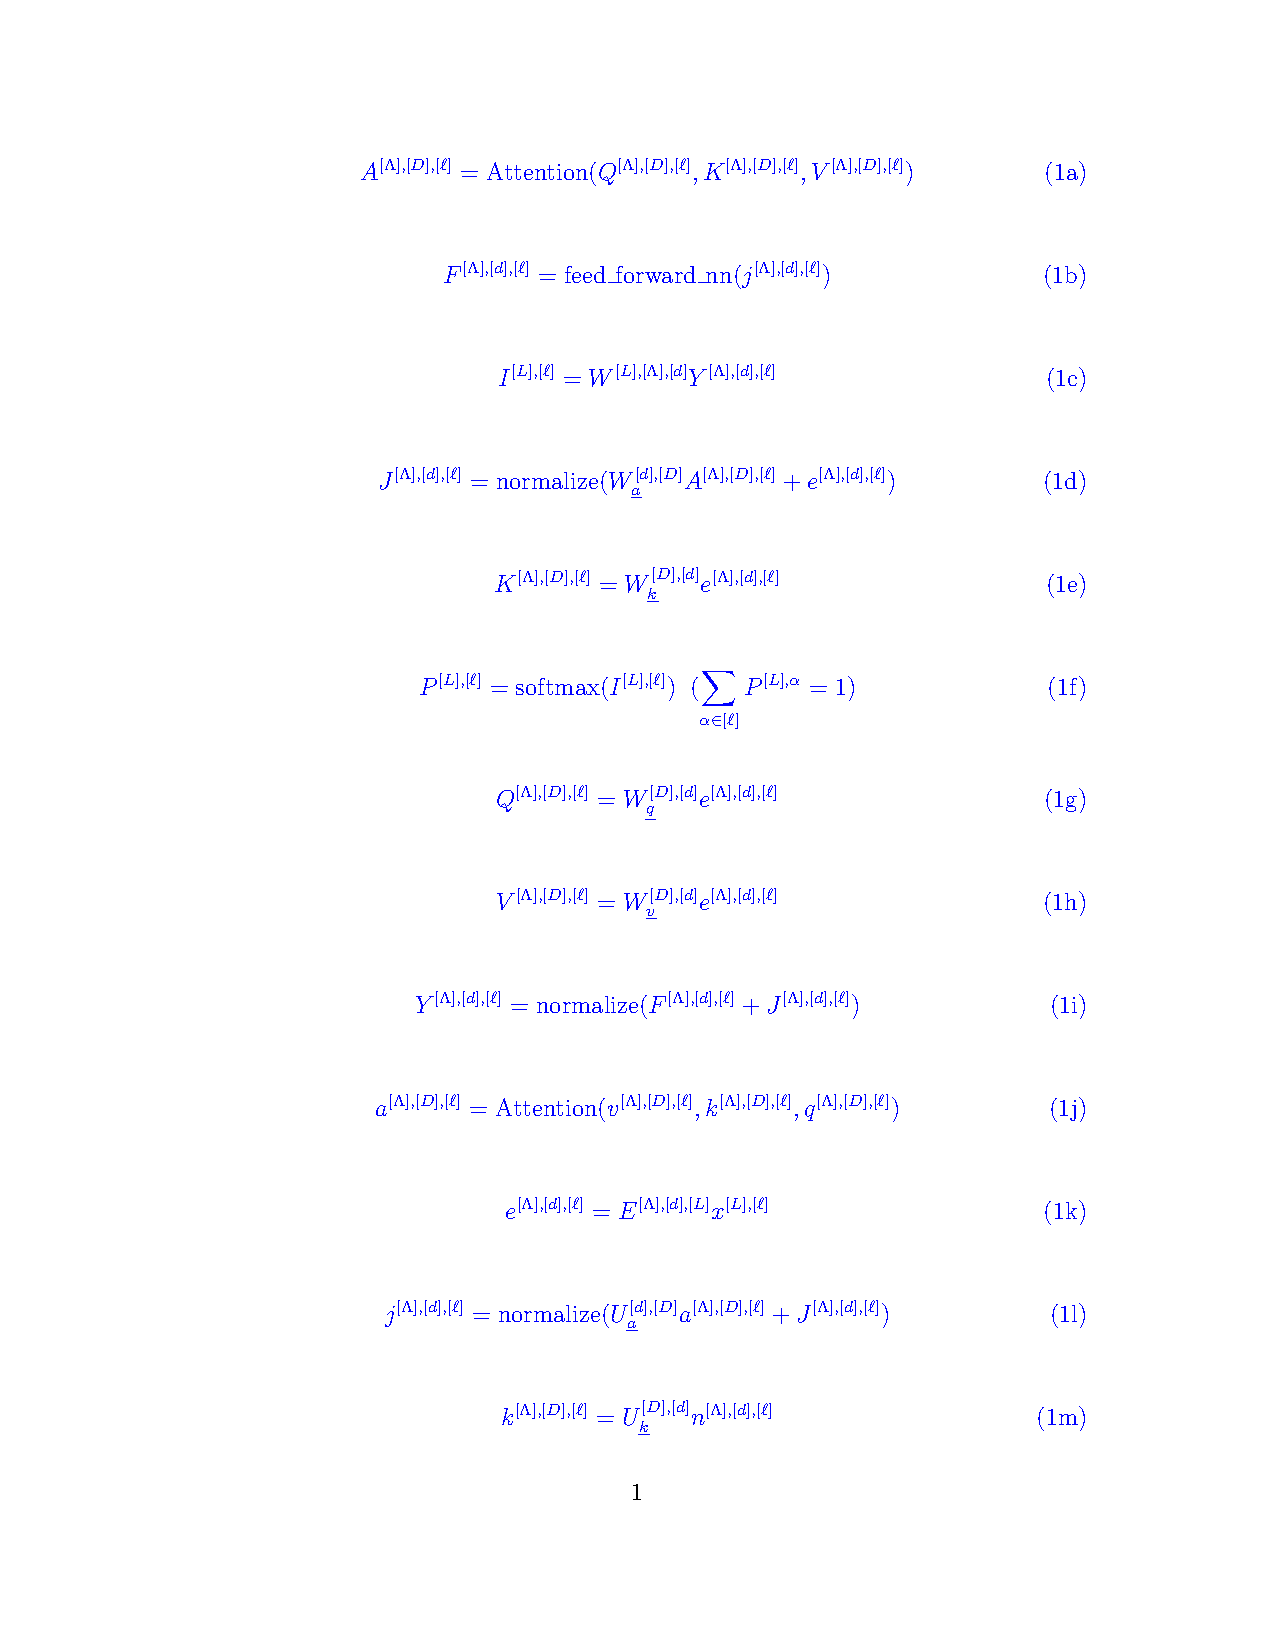
\includegraphics[width=2in]{decoder.jpg}
\end{minipage}%blank lines between minispaces breaks this
\begin{minipage}{.6\linewidth}
$$\xymatrix@R=2pc@C=0.2pc{
&&&*+[F*:SpringGreen]{\underline{P}^{[L],[\ell]}}
\\
&&&*+[F*:Orchid]{\underline{I}^{[L],[\ell]}}\ar[u]
\\
&&&*+[F*:yellow]{\underline{Y}^{[d], [\ell]}}\ar[u]
\\
&&*+[F*:SkyBlue]{\underline{F}^{[d], [\ell]}}\ar[ur]&
\\
&*+[F*:Dandelion]{\underline{a}^{[D],[\ell]}}\ar[rr]^{U_\rva}&&*+[F*:yellow]{\underline{j}^{[d], [\ell]}}\ar[ul]\ar[uu]
\\
*+[F*:Dandelion]{\underline{v}^{[D], [\ell]}}\ar[ur]&*+[F*:Dandelion]{\underline{k}^{[D], [\ell]}}\ar[u]&*+[F*:Dandelion]{\underline{q}^{[D], [\ell]}}\ar[ul]&
\\
*+[F*:yellow]{\underline{n}^{[d], [\ell]}}\ar[ur]_{U_\rvk}\ar[u]^{U_\rvv}&&&*+[F*:yellow]{\underline{J}^{[d], [\ell]}}\ar[uu]\ar[ul]^{U_\rvq}
\\
&*+[F*:Dandelion]{\underline{A}^{[D],[\ell]}}\ar[urr]^{W_\rva}&&
\\
*+[F*:Dandelion]{\underline{Q}^{[D], [\ell]}}\ar[ur]&*+[F*:Dandelion]{\underline{K}^{[D], [\ell]}}\ar[u]&*+[F*:Dandelion]{\underline{V}^{[D], [\ell]}}\ar[ul]&
\\
&&&
\\
&&&*+[F*:gray]{\underline{e}^{[d],[\ell]}}\ar[uuuu]\ar[uull]_{W_\rvk}\ar[uulll]^{W_\rvq}\ar[uul]_{W_\rvv}
\\
&&&*+[F*:Lavender]{\underline{x}^{[L],[\ell]}}\ar[u]
\save
\POS"3,1"."9,1"."3,4"."9,4"!C*+<7.5em>\frm{-,}
\restore
}$$
\end{minipage}
\caption{Decoder of Vanilla Transformer Net. $\Lam$ copies of the boxed part are connected in series.}
\label{fig-texnn-for-decoder}
\end{figure}

\begin{subequations}

\begin{equation}\color{blue}
A^{[D],[\ell]} = \text{Attention}(Q^{[D], [\ell]},K^{[D], [\ell]},V^{[D], [\ell]})
\label{eq-o-fun-decoder}
\end{equation}

\begin{equation}\color{blue}
F^{[d], [\ell]} = \text{feed\_forward\_nn}(j^{[d], [\ell]})
\label{eq-B-fun-decoder}
\end{equation}

\begin{equation}\color{blue}
I^{[L],[\ell]} = W^{[L], [d]}Y^{[d], [\ell]}
\label{eq-I-fun-decoder}
\end{equation}

\begin{equation}\color{blue}
J^{[d], [\ell]} = \text{normalize}(W_\rva^{[d], [D]}A^{[D],[\ell]} + e^{[d],[\ell]})
\label{eq-a-fun-decoder}
\end{equation}

\begin{equation}\color{blue}
K^{[D], [\ell]} = W_\rvk^{[D],[d]}e^{[d],[\ell]}
\label{eq-K-fun-decoder}
\end{equation}

\begin{equation}\color{blue}
P^{[L],[\ell]} = \text{softmax}(I^{[L],[\ell]})\;\;\text{$(\sum_{\alp\in[\ell]}P^{[L], \alp}=1)$}
\label{eq-G-fun-decoder}
\end{equation}

\begin{equation}\color{blue}
Q^{[D], [\ell]} = W_\rvq^{[D],[d]}e^{[d],[\ell]}
\label{eq-Q-fun-decoder}
\end{equation}

\begin{equation}\color{blue}
V^{[D], [\ell]} = W_\rvv^{[D],[d]}e^{[d],[\ell]}
\label{eq-V-fun-decoder}
\end{equation}

\begin{equation}\color{blue}
Y^{[d], [\ell]} = \text{normalize}(F^{[d], [\ell]} + J^{[d], [\ell]})
\label{eq-Y-fun-decoder}
\end{equation}

\begin{equation}\color{blue}
a^{[D],[\ell]} = \text{Attention}(v^{[D], [\ell]},k^{[D], [\ell]},q^{[D], [\ell]})
\label{eq-O-fun-decoder}
\end{equation}

\begin{equation}\color{blue}
e^{[d],[\ell]} = E^{[d],[L]}x^{[L],[\ell]}
\label{eq-p-fun-decoder}
\end{equation}

\begin{equation}\color{blue}
j^{[d], [\ell]} = \text{normalize}(U_\rva^{[d],[D]}a^{[D],[\ell]} + J^{[d], [\ell]})
\label{eq-j-fun-decoder}
\end{equation}

\begin{equation}\color{blue}
k^{[D], [\ell]} = U_\rvk^{[D],[d]}n^{[d], [\ell]}
\label{eq-k-fun-decoder}
\end{equation}

\begin{equation}\color{blue}
n^{[d], [\ell]} = \;\;\text{Prior coming from Encoder.}
\label{eq-n-fun-decoder}
\end{equation}

\begin{equation}\color{blue}
q^{[D], [\ell]} = U_\rvq^{[D],[d]}J^{[d], [\ell]}
\label{eq-q-fun-decoder}
\end{equation}

\begin{equation}\color{blue}
v^{[D], [\ell]} = U_\rvv^{[D], [d]}n^{[d], [\ell]}
\label{eq-v-fun-decoder}
\end{equation}

\begin{equation}\color{blue}
x^{[L],[\ell]} = \;\;\text{prior, right shifted output}
\label{eq-R-fun-decoder}
\end{equation}

\end{subequations}


\end{document}  
